%% Screen version %%%%%%%%%%%%%%%%%%%%%%%%%%%%%%%%%%%%%%%%%%%%%%%%%%%%%%%%%%%%%%
\documentclass[xcolor=x11names,compress]{beamer}

% Handout version %%%%%%%%%%%%%%%%%%%%%%%%%%%%%%%%%%%%%%%%%%%%%%%%%%%%%%%%%%%%%%
%\documentclass[xcolor=x11names,compress,handout]{beamer}
%
%\usepackage{pgfpages}
%\pgfpagesuselayout{4 on 1}[a4paper,landscape,border shrink=5mm]

% Ładniejsze tabelki
\usepackage{booktabs}

%% General document %%%%%%%%%%%%%%%%%%%%%%%%%%%%%%%%%%%%%%%%%%%%%%%%%%%%%%%%%%%%
\usepackage{graphicx}
\usepackage[MeX]{polski}

\usepackage[absolute]{textpos}

\usepackage{fancybox}

\usepackage[utf8]{inputenc}
\usepackage{tikz}
\usetikzlibrary{decorations.fractals}
%%%%%%%%%%%%%%%%%%%%%%%%%%%%%%%%%%%%%%%%%%%%%%%%%%%%%%%%%%%%%%%%%%%%%%%%%%%%%%%%


%% Beamer Layout %%%%%%%%%%%%%%%%%%%%%%%%%%%%%%%%%%%%%%%%%%%%%%%%%%%%%%%%%%%%%%%
\useoutertheme[subsection=false,shadow,footline=authortitle]{miniframes}
\useinnertheme{default}
\usefonttheme{serif}
\usepackage[T1]{fontenc}
\usepackage{palatino}

\setbeamerfont{title like}{shape=\scshape}
\setbeamerfont{frametitle}{shape=\scshape}

\setbeamercolor*{lower separation line head}{bg=DeepSkyBlue4}
\setbeamercolor*{upper separation line foot}{bg=DeepSkyBlue4}
\setbeamercolor*{normal text}{fg=black,bg=white}
\setbeamercolor*{alerted text}{fg=DeepSkyBlue4}
\setbeamercolor*{example text}{fg=black}
\setbeamercolor*{structure}{fg=DeepSkyBlue4}
\setbeamercolor*{itemize item}{fg=DeepSkyBlue4}

\setbeamercolor*{palette tertiary}{fg=black,bg=black!10}
\setbeamercolor*{palette quaternary}{fg=black,bg=black!10}

\setbeamersize{
  text margin left=1cm,
  text margin right=1cm
}

\newcommand{\code}[1]{\textit{#1}}

\renewcommand{\(}{\begin{columns}}
\renewcommand{\)}{\end{columns}}
\newcommand{\<}[1]{\begin{column}{#1}}
\renewcommand{\>}{\end{column}}

% definicja symboli do tabeli cech
\def\YES{\CIRCLE}        % posiada
\def\HALF{\LEFTcircle}   % częściowo posiada
\def\NO{\Circle}         % nie posiada
\def\NA{$\times$}          % nie dotyczy


%%%%%%%%%%%%%%%%%%%%%%%%%%%%%%%%%%%%%%%%%%%%%%%%%%%%%%%%%%%%%%%%%%%%%%%%%%%%%%%%

\setcounter{tocdepth}{2}

% The following command gets rid of the navigation symbols that you usually
% see at the bottom-right of people's Beamer talks.
%
\setbeamertemplate{navigation symbols}{}

\setbeamercovered{transparent}

\begin{document}

\title{Wykorzystanie informacji z kamery 3D\\ do nawigacji robota mobilnego}
\author{Maciej Stefańczyk}
\institute{\it Wydział Elektroniki i Technik Informacyjnych Politechniki Warszawskiej}
\date{
	\begin{figure}[h!]
	\centering
	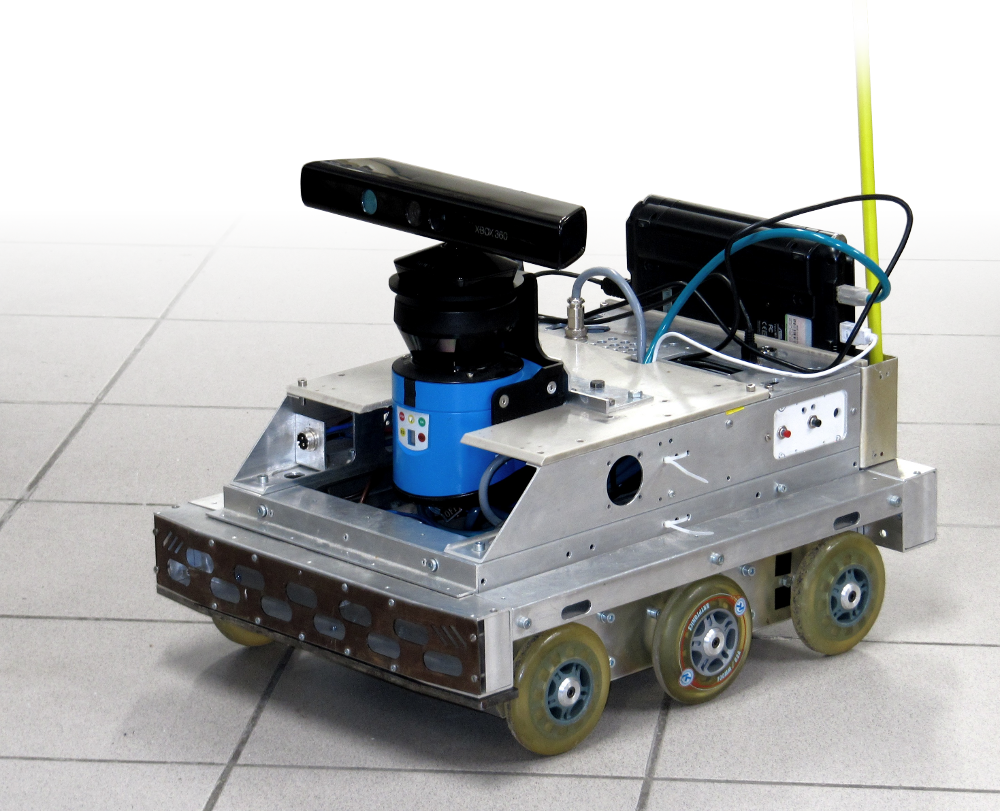
\includegraphics[width=4.4cm]{../Common/img/elektron/elektron_kinect}
	\label{fig:p1}
	\end{figure}

	\vspace{.0cm}
	8 września 2011
}

\AtBeginSection[]
{
  \begin{frame}<beamer>
    \frametitle{Plan prezentacji}
    \tableofcontents[currentsection]
  \end{frame}
}

%%%%%%%%%%%%%%%%%%%%%%%%%%%%%%%%%%%%%%%%%%%%%%%%%%%%%%%%%%%%%%%%%%%%%%%%%%%%%%%%
%%%%%%%%%%%%%%%%%%%%%%%%%%%%%%%%%%%%%%%%%%%%%%%%%%%%%%%%%%%%%%%%%%%%%%%%%%%%%%%%

\setbeamercolor{normal text}{bg=black!10}

\begin{frame}[plain]

\titlepage
\end{frame}

\setbeamercolor{normal text}{bg=}

%%%%%%%%%%%%%%%%%%%%%%%%%%%%%%%%%%%%%%%%%%%%%%%%%%%%%%%%%%%%%%%%%%%%%%%%%%%%%%%%
%%%%%%%%%%%%%%%%%%%%%%%%%%%%%%%%%%%%%%%%%%%%%%%%%%%%%%%%%%%%%%%%%%%%%%%%%%%%%%%%
\begin{frame}{Plan prezentacji}
	\frametitle{Plan prezentacji}
	\tableofcontents
\end{frame}

%%%%%%%%%%%%%%%%%%%%%%%%%%%%%%%%%%%%%%%%%%%%%%%%%%%%%%%%%%%%%%%%%%%%%%%%%%%%%%%%
%%%%%%%%%%%%%%%%%%%%%%%%%%%%%%%%%%%%%%%%%%%%%%%%%%%%%%%%%%%%%%%%%%%%%%%%%%%%%%%%

\section{\scshape Wprowadzenie}
\subsection{Motywacja}

\begin{frame}{Motywacja}

\alert{Problemy z klasycznymi czujnikami wykrywania przeszkód:}
\begin{itemize}
\item małe przeszkody leżące na ziemi,
\item elementy otoczenia zwisające nad robotem,
\item wykrywanie spadków terenu.
\end{itemize}

\vspace{.5cm}

\alert{Problem testowania systemów robotycznych:}
\begin{itemize}
\item bezpieczeństwo,
\item dobór parametrów.
\end{itemize}

\end{frame}

%%%%%%%%%%%%%%%%%%%%%%%%%%%%%%%%%%%%%%%%%%%%%%%%%%%%%%%%%%%%%%%%%%%%%%%%%%%%%%%%
%%%%%%%%%%%%%%%%%%%%%%%%%%%%%%%%%%%%%%%%%%%%%%%%%%%%%%%%%%%%%%%%%%%%%%%%%%%%%%%%
\subsection{Cel pracy}

\begin{frame}{Cel pracy}

\alert{Wykorzystanie kamery 3D:}
\begin{itemize}
\item wybór odpowiedniego rozwiązania,
\item przetwarzanie danych o otoczeniu.
\end{itemize}

\vspace{.5cm}

\alert{System nawigacji:}
\begin{itemize}
\item gotowe do wykorzystania stanowisko eksperymentalne,
\item budowa modułowa.
\end{itemize}

\end{frame}

%%%%%%%%%%%%%%%%%%%%%%%%%%%%%%%%%%%%%%%%%%%%%%%%%%%%%%%%%%%%%%%%%%%%%%%%%%%%%%%%
%%%%%%%%%%%%%%%%%%%%%%%%%%%%%%%%%%%%%%%%%%%%%%%%%%%%%%%%%%%%%%%%%%%%%%%%%%%%%%%%
\section{\scshape Wykorzystanie kamery 3D}
\subsection{Źródła obrazu 3D}
\begin{frame}{Wykorzystanie czujników odległości}

\alert{Działanie:}
\begin{itemize}
\item czujniki umieszczone na\\ruchomych głowicach,
\item skanowanie sekwencyjne.
\end{itemize}

\vspace{.5cm}

\alert{Zalety:}
\begin{itemize}
\item łatwe przetwarzanie wyników,
\item dostępność czujników.
\end{itemize}

\vspace{.5cm}

\alert{Wady:}
\begin{itemize}
\item wymagane środowisko statyczne,
\item szybkość działania.
\end{itemize}

\begin{textblock*}{50mm}(75mm,15mm)%
%  \noindent\colorbox[rgb]{0,1,0}{%
    \begin{minipage}[l]{50mm}%

	\begin{figure}[h!]
    \centering
    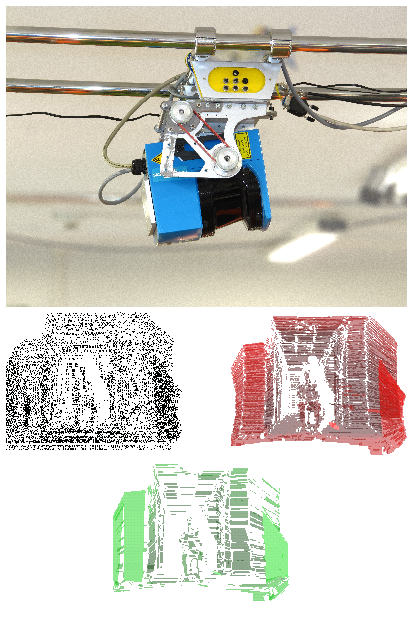
\includegraphics[width=5.0cm]{../Common/img/sick_vert}
    \end{figure}

    \end{minipage}
%  }%
\end{textblock*}

\end{frame}

%%%%%%%%%%%%%%%%%%%%%%%%%%%%%%%%%%%%%%%%%%%%%%%%%%%%%%%%%%%%%%%%%%%%%%%%%%%%%%%%
%%%%%%%%%%%%%%%%%%%%%%%%%%%%%%%%%%%%%%%%%%%%%%%%%%%%%%%%%%%%%%%%%%%%%%%%%%%%%%%%
\begin{frame}{Stereowizja}

\alert{Działanie:}
\begin{itemize}
\item korelacja obrazów \\z dwóch kamer,
\item wyszukiwanie punktów \\charakterystycznych.
\end{itemize}

\vspace{.2cm}

\alert{Zalety:}
\begin{itemize}
\item dostępność sprzętu,
\item działanie na obszarach otwartych.
\end{itemize}

\vspace{.2cm}

\alert{Wady:}
\begin{itemize}
\item obiekty jednolite,
\item jakość kamer.
\end{itemize}

\begin{textblock*}{50mm}(75mm,15mm)%
%  \noindent\colorbox[rgb]{0,1,0}{%
    \begin{minipage}[l]{50mm}%

	\begin{figure}[h!]
    \centering
    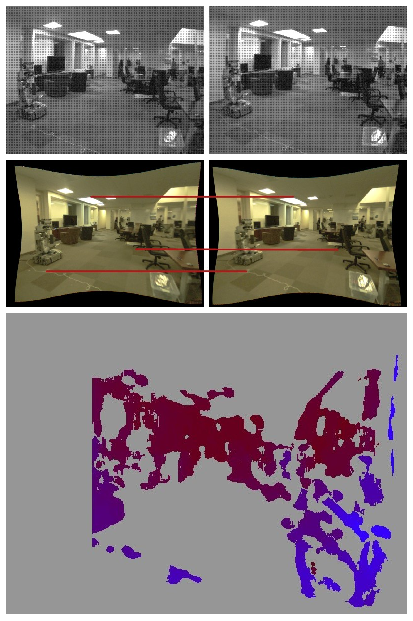
\includegraphics[width=5.0cm]{../Common/img/stereo_steps_vert}
    \end{figure}

    \end{minipage}
%  }%
\end{textblock*}

\end{frame}

%%%%%%%%%%%%%%%%%%%%%%%%%%%%%%%%%%%%%%%%%%%%%%%%%%%%%%%%%%%%%%%%%%%%%%%%%%%%%%%%
%%%%%%%%%%%%%%%%%%%%%%%%%%%%%%%%%%%%%%%%%%%%%%%%%%%%%%%%%%%%%%%%%%%%%%%%%%%%%%%%
\begin{frame}{Kamery TOF}

\alert{Działanie:}
\begin{itemize}
\item oświetlenie sceny i pomiar czasu powrotu światła.
\end{itemize}

\vspace{.4cm}

\alert{Zalety:}
\begin{itemize}
\item szybkość działania,
\item dokładność pokrycia.
\end{itemize}

\vspace{.4cm}

\alert{Wady:}
\begin{itemize}
\item drogi sprzęt,
\item niska rozdzielczość,
\item interferencje.
\end{itemize}

\end{frame}

%%%%%%%%%%%%%%%%%%%%%%%%%%%%%%%%%%%%%%%%%%%%%%%%%%%%%%%%%%%%%%%%%%%%%%%%%%%%%%%%
%%%%%%%%%%%%%%%%%%%%%%%%%%%%%%%%%%%%%%%%%%%%%%%%%%%%%%%%%%%%%%%%%%%%%%%%%%%%%%%%
\begin{frame}{Światło strukturalne}

\alert{Działanie:}
\begin{itemize}
\item rzutowanie wzorca \\i analiza obrazu,
\item różne wzorce.
\end{itemize}

\vspace{.2cm}

\alert{Zalety:}
\begin{itemize}
\item dobre pokrycie,
\item sceny statyczne i dynamiczne.
\end{itemize}

\vspace{.2cm}

\alert{Wady:}
\begin{itemize}
\item problemy na zewnątrz,
\item dodatkowy osprzęt.
\end{itemize}

\begin{textblock*}{50mm}(75mm,15mm)%
%  \noindent\colorbox[rgb]{0,1,0}{%
    \begin{minipage}[l]{50mm}%

	\begin{figure}[h!]
    \centering
    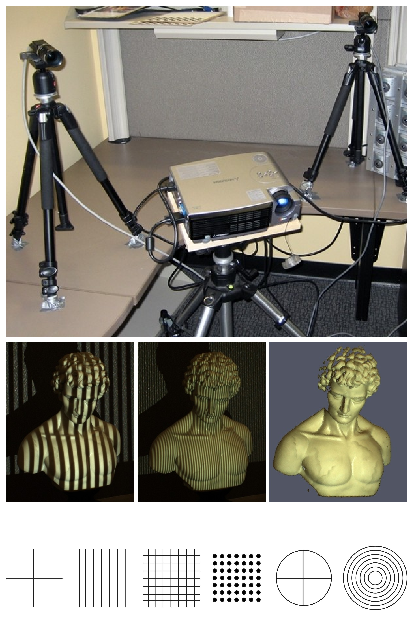
\includegraphics[width=5.0cm]{../Common/img/struct_vert}
    \end{figure}

    \end{minipage}
%  }%
\end{textblock*}

\end{frame}

%%%%%%%%%%%%%%%%%%%%%%%%%%%%%%%%%%%%%%%%%%%%%%%%%%%%%%%%%%%%%%%%%%%%%%%%%%%%%%%%
%%%%%%%%%%%%%%%%%%%%%%%%%%%%%%%%%%%%%%%%%%%%%%%%%%%%%%%%%%%%%%%%%%%%%%%%%%%%%%%%
\subsection{Porównanie wybranych rozwiązań}

\begin{frame}{Porównanie wybranych rozwiązań}

\begin{figure}[h!]
\centering
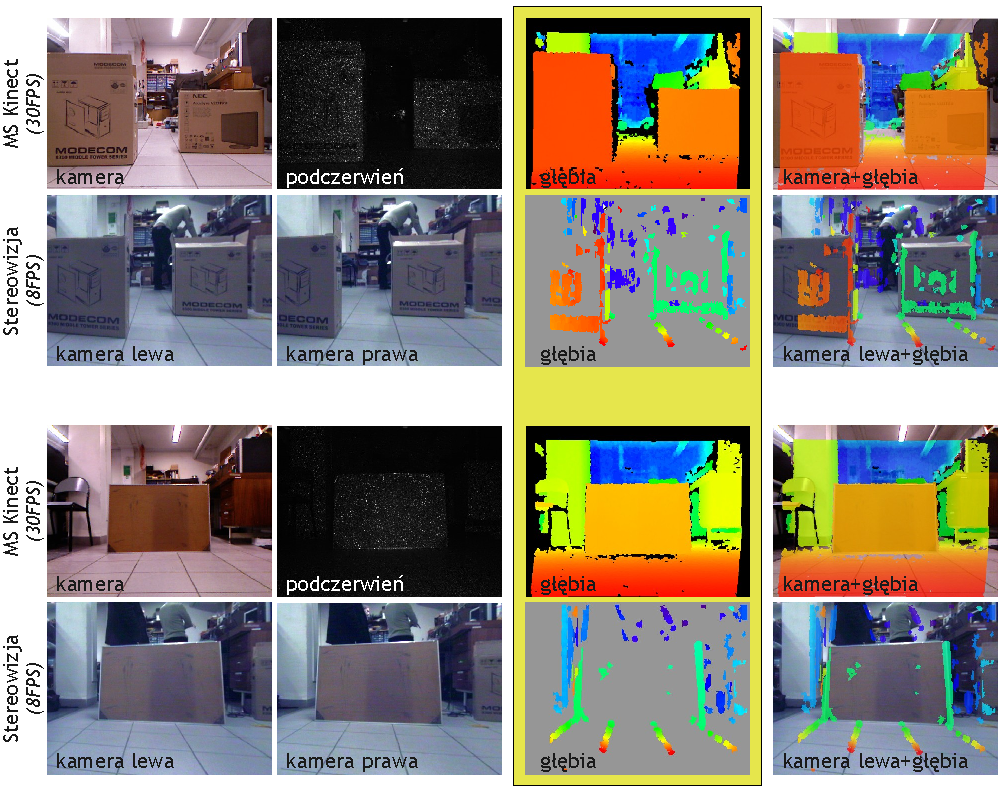
\includegraphics[width=9.5cm]{../Common/img/compare}
\end{figure}

\end{frame}

%%%%%%%%%%%%%%%%%%%%%%%%%%%%%%%%%%%%%%%%%%%%%%%%%%%%%%%%%%%%%%%%%%%%%%%%%%%%%%%%
%%%%%%%%%%%%%%%%%%%%%%%%%%%%%%%%%%%%%%%%%%%%%%%%%%%%%%%%%%%%%%%%%%%%%%%%%%%%%%%%
%%%%%%%%%%%%%%%%%%%%%%%%%%%%%%%%%%%%%%%%%%%%%%%%%%%%%%%%%%%%%%%%%%%%%%%%%%%%%%%%
%%%%%%%%%%%%%%%%%%%%%%%%%%%%%%%%%%%%%%%%%%%%%%%%%%%%%%%%%%%%%%%%%%%%%%%%%%%%%%%%
\section{\scshape Zrealizowany system nawigacji}
\subsection{Dekompozycja zadania}
\begin{frame}{Dekompozycja zadania}

\alert{Podział na odrębne moduły:}
\begin{itemize}
\item zmniejszenie zależności,
\item wymienność elementów,
\item elastyczność zastosowania.
\end{itemize}

\vspace{.2cm}

\alert{Wykorzysanie elementów istniejących:}
\begin{itemize}
\item niektóre algorytmy,
\item struktura systemu nawigacji.
\end{itemize}

\vspace{.2cm}

\alert{Implementacja nowych modułów:}
\begin{itemize}
\item filtrowanie danych,
\item sterowanie bazą jezdną,
\item diagnostyka.
\end{itemize}

\begin{textblock*}{70mm}(65mm,10mm)%
%  \noindent\colorbox[rgb]{0,1,0}{%
    \begin{minipage}[l]{70mm}%

	\begin{figure}[h!]
    \centering
    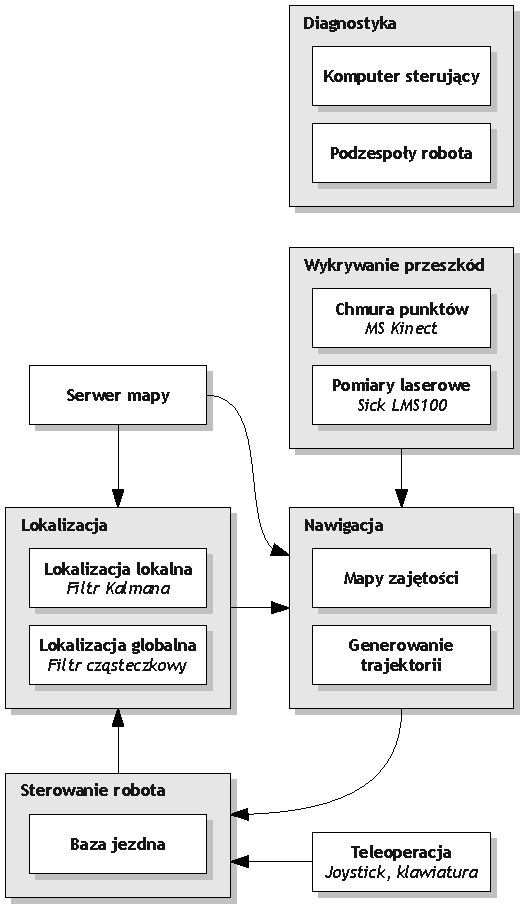
\includegraphics[width=4.2cm]{../MSc/img/decomposition_vert}
    \end{figure}
    \end{minipage}
%  }%
\end{textblock*}

\hspace{3.5cm} \scriptsize \alert{Rysunek:} Najważniejsze moduły stworzonej platformy.

\end{frame}

%%%%%%%%%%%%%%%%%%%%%%%%%%%%%%%%%%%%%%%%%%%%%%%%%%%%%%%%%%%%%%%%%%%%%%%%%%%%%%%%
%%%%%%%%%%%%%%%%%%%%%%%%%%%%%%%%%%%%%%%%%%%%%%%%%%%%%%%%%%%%%%%%%%%%%%%%%%%%%%%%
\subsection{Struktura systemu nawigacji}

\begin{frame}{Struktura systemu nawigacji}

\alert{Wymienność modułów:}
\begin{itemize}
\item planowanie trasy,
\item zachowania ratunkowe,
\item lokalizacja,
\item akwizycja danych sensorycznych.
\end{itemize}

\vspace{.5cm}

\alert{Elastyczność:}
\begin{itemize}
\item możliwość wykorzystania\\jedynie niektórych\\modułów,
\item abstrakcja danych.
\end{itemize}

\begin{textblock*}{70mm}(60mm,18mm)%
    \begin{minipage}[c]{70mm}%
	\begin{figure}[h!]
	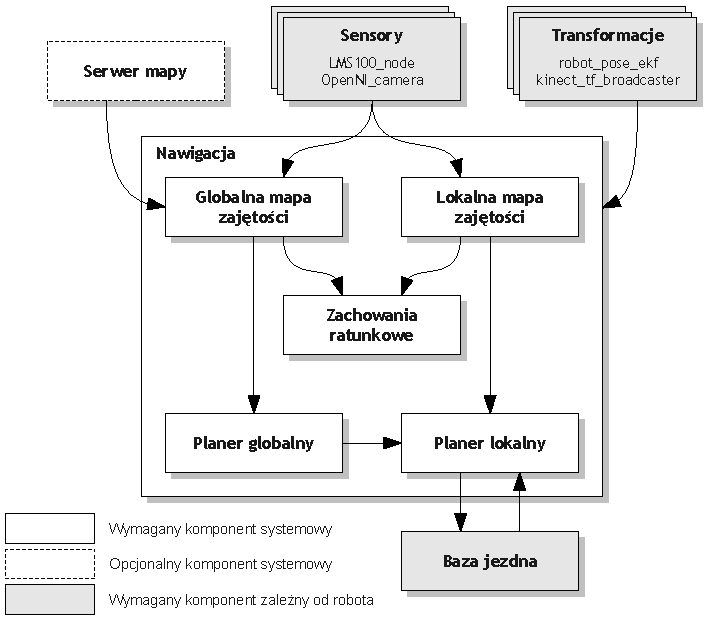
\includegraphics[width=5.2cm]{../MSc/img/diag_move_base}
	\end{figure}
	\hspace{1cm}\scriptsize \alert{Rysunek:} Struktura i zależności modułu

	\hspace{1cm}nawigacyjnego.
    \end{minipage}
\end{textblock*}

\end{frame}

%%%%%%%%%%%%%%%%%%%%%%%%%%%%%%%%%%%%%%%%%%%%%%%%%%%%%%%%%%%%%%%%%%%%%%%%%%%%%%%%
%%%%%%%%%%%%%%%%%%%%%%%%%%%%%%%%%%%%%%%%%%%%%%%%%%%%%%%%%%%%%%%%%%%%%%%%%%%%%%%%
\begin{frame}{Lokalizacja i tworzenie map przeszkód}

\alert{Lokalizacja:}
\begin{itemize}
\item mapa otoczenia,
\item odczyty z odometrii,
\item żyroskop.
\end{itemize}

\vspace{1cm}

\alert{Mapa zajętości:}
\begin{itemize}
\item filtrowanie danych,
\item czyszczenie,
\item oznaczanie przeszkód,
\item zachowania ratunkowe.
\end{itemize}



\begin{textblock*}{70mm}(60mm,25mm)%
%  \noindent\colorbox[rgb]{0,1,0}{%
    \begin{minipage}[l]{70mm}%

	\begin{figure}[h!]
	\centering
	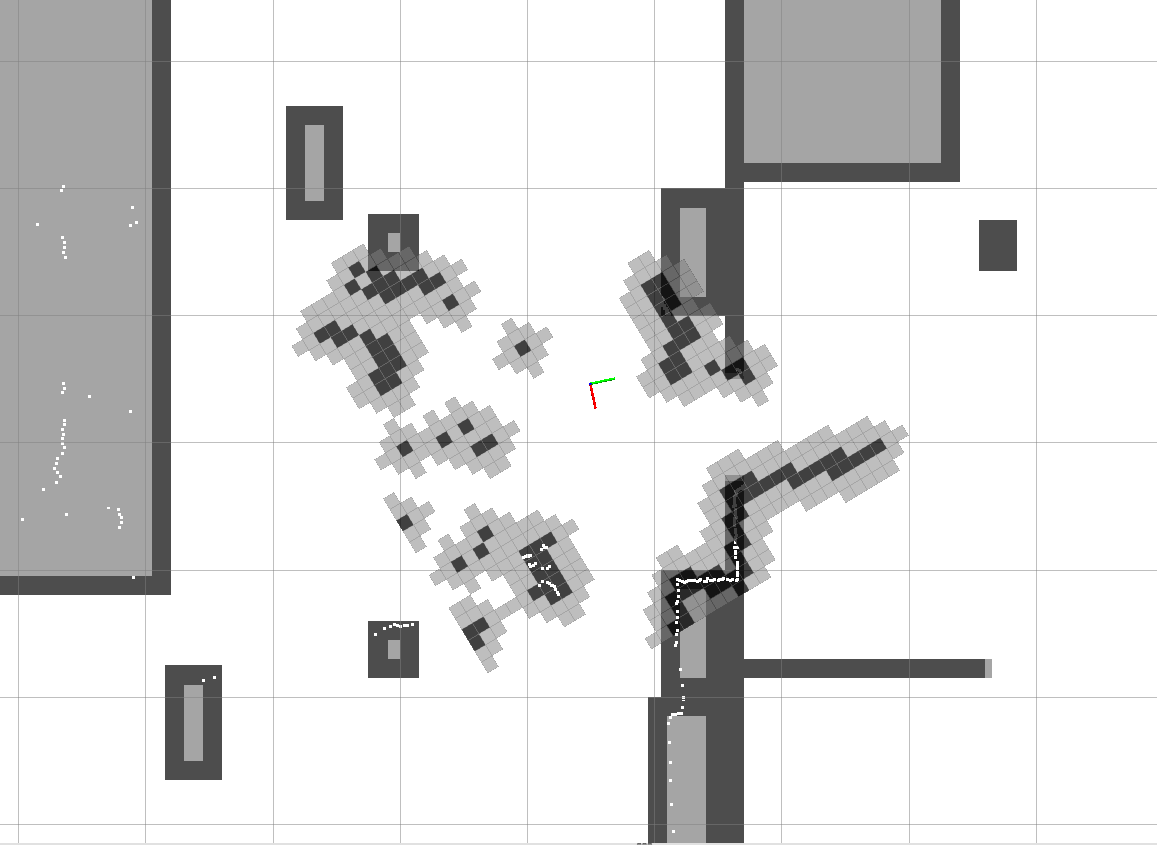
\includegraphics[width=5.2cm]{../MSc/img/costmap}
	\end{figure}

	\hspace{1cm}\scriptsize \alert{Rysunek:} Fragment mapy globalnej

	\hspace{1cm}oraz lokalna mapa zajętości.
    \end{minipage}
%  }%
\end{textblock*}

\end{frame}

%%%%%%%%%%%%%%%%%%%%%%%%%%%%%%%%%%%%%%%%%%%%%%%%%%%%%%%%%%%%%%%%%%%%%%%%%%%%%%%%
%%%%%%%%%%%%%%%%%%%%%%%%%%%%%%%%%%%%%%%%%%%%%%%%%%%%%%%%%%%%%%%%%%%%%%%%%%%%%%%%
\begin{frame}{Planowanie trasy i omijanie przeszkód}

\alert{Planowanie trasy:}
\begin{itemize}
\item off-line,
\item mapa globalna,
\item uogólnienia dot. kształtu.
\end{itemize}

\vspace{.7cm}

\alert{Omijanie przeszkód:}
\begin{itemize}
\item on-line,
\item otoczenie robota,
\item uwzględniona kinematyka robota,
\item dokładny model robota.
\end{itemize}

\end{frame}

%%%%%%%%%%%%%%%%%%%%%%%%%%%%%%%%%%%%%%%%%%%%%%%%%%%%%%%%%%%%%%%%%%%%%%%%%%%%%%%%
%%%%%%%%%%%%%%%%%%%%%%%%%%%%%%%%%%%%%%%%%%%%%%%%%%%%%%%%%%%%%%%%%%%%%%%%%%%%%%%%
%%%%%%%%%%%%%%%%%%%%%%%%%%%%%%%%%%%%%%%%%%%%%%%%%%%%%%%%%%%%%%%%%%%%%%%%%%%%%%%%
%%%%%%%%%%%%%%%%%%%%%%%%%%%%%%%%%%%%%%%%%%%%%%%%%%%%%%%%%%%%%%%%%%%%%%%%%%%%%%%%
\section{\scshape Eksperymenty}

%%%%%%%%%%%%%%%%%%%%%%%%%%%%%%%%%%%%%%%%%%%%%%%%%%%%%%%%%%%%%%%%%%%%%%%%%%%%%%%%
%%%%%%%%%%%%%%%%%%%%%%%%%%%%%%%%%%%%%%%%%%%%%%%%%%%%%%%%%%%%%%%%%%%%%%%%%%%%%%%%
\subsection*{}
\begin{frame}{Wykorzystanie symulacji}


\alert{Możliwości:}
\begin{itemize}
\item dobór parametrów,
\item sprawdzenie poprawności \\koncepcji,
\item testy niektórych algorytmów.
\end{itemize}

\vspace{.7cm}

\alert{Problemy:}
\begin{itemize}
\item modelowanie czujników,
\item brak ,,naturalnych'' zachowań,
\item odwzorowanie środowiska.
\end{itemize}

\begin{textblock*}{70mm}(60mm,18mm)%
    \begin{minipage}[c]{70mm}%
	\begin{figure}[h!]
	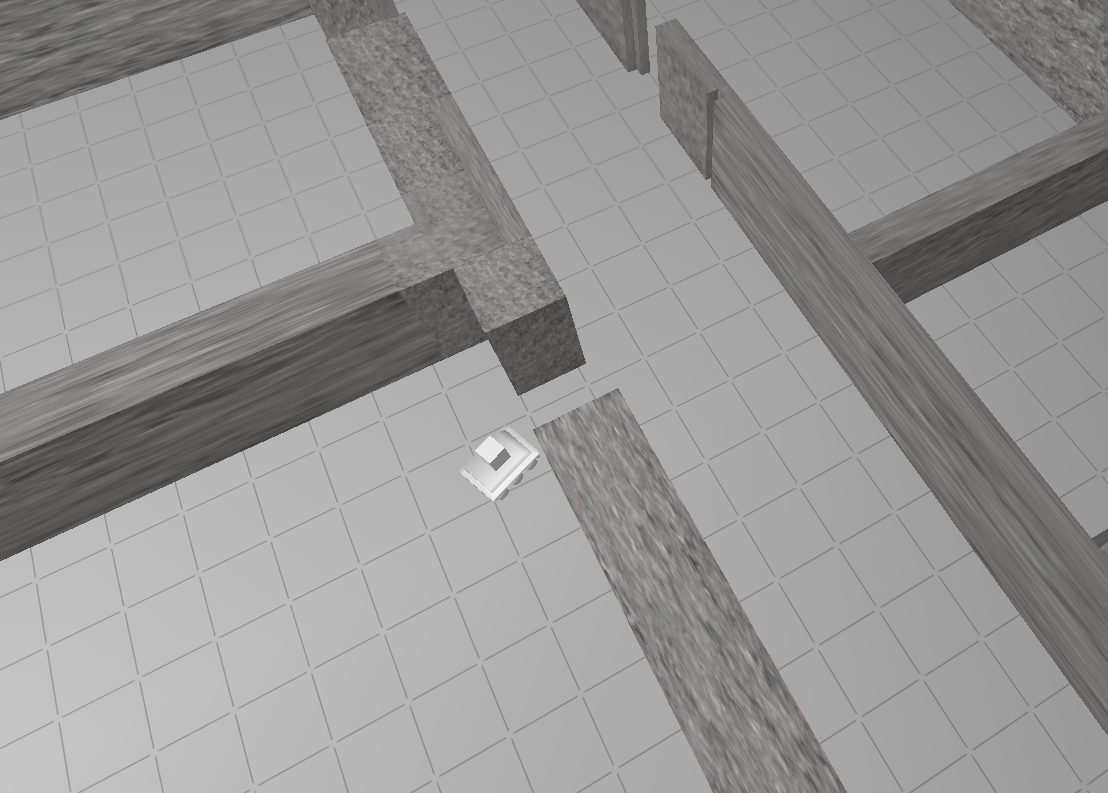
\includegraphics[width=5.2cm]{../MSc/img/gazebo}
	\end{figure}
	\hspace{1cm}\scriptsize \alert{Rysunek:} Robot Elektron w symulatorze.
    \end{minipage}
\end{textblock*}

\end{frame}

%%%%%%%%%%%%%%%%%%%%%%%%%%%%%%%%%%%%%%%%%%%%%%%%%%%%%%%%%%%%%%%%%%%%%%%%%%%%%%%%
%%%%%%%%%%%%%%%%%%%%%%%%%%%%%%%%%%%%%%%%%%%%%%%%%%%%%%%%%%%%%%%%%%%%%%%%%%%%%%%%
\begin{frame}{Testy w kontrolowanych warunkach}

\alert{Możliwości:}
\begin{itemize}
\item ostateczne dopasowanie \\parametrów,
\item aranżacja zagrożeń,
\item naturalne zachowania.
\end{itemize}

\vspace{.7cm}

\alert{Problemy:}
\begin{itemize}
\item ,,bezpieczne'' ruchy,
\item zabezpieczenie robota,
\item destrukcja otoczenia.
\end{itemize}

\begin{textblock*}{70mm}(60mm,18mm)%
    \begin{minipage}[c]{70mm}%
	\begin{figure}[h!]
	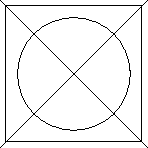
\includegraphics[width=5.2cm]{../Common/img/placeholder}
	\end{figure}
	\hspace{1cm}\scriptsize \alert{Rysunek:} Przejazdy testowe.
    \end{minipage}
\end{textblock*}

\end{frame}

%%%%%%%%%%%%%%%%%%%%%%%%%%%%%%%%%%%%%%%%%%%%%%%%%%%%%%%%%%%%%%%%%%%%%%%%%%%%%%%%
%%%%%%%%%%%%%%%%%%%%%%%%%%%%%%%%%%%%%%%%%%%%%%%%%%%%%%%%%%%%%%%%%%%%%%%%%%%%%%%%
\begin{frame}{Testy w docelowym środowisku}

\alert{Możliwości:}
\begin{itemize}
\item potwierdzenie prawidłowości \\działania,
\item pełna gama sytuacji \\wyjątkowych.
\end{itemize}

\vspace{.7cm}

\alert{Problemy:}
\begin{itemize}
\item wpływ otoczenia,
\item uwzgędnione w algorytmach.
\end{itemize}

\begin{textblock*}{70mm}(60mm,18mm)%
    \begin{minipage}[c]{70mm}%
	\begin{figure}[h!]
	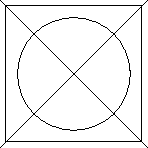
\includegraphics[width=5.2cm]{../Common/img/placeholder}
	\end{figure}
	\hspace{1cm}\scriptsize \alert{Rysunek:} Działanie w otoczeniu docelowym.
    \end{minipage}
\end{textblock*}

\end{frame}

%%%%%%%%%%%%%%%%%%%%%%%%%%%%%%%%%%%%%%%%%%%%%%%%%%%%%%%%%%%%%%%%%%%%%%%%%%%%%%%%
%%%%%%%%%%%%%%%%%%%%%%%%%%%%%%%%%%%%%%%%%%%%%%%%%%%%%%%%%%%%%%%%%%%%%%%%%%%%%%%%
%%%%%%%%%%%%%%%%%%%%%%%%%%%%%%%%%%%%%%%%%%%%%%%%%%%%%%%%%%%%%%%%%%%%%%%%%%%%%%%%
%%%%%%%%%%%%%%%%%%%%%%%%%%%%%%%%%%%%%%%%%%%%%%%%%%%%%%%%%%%%%%%%%%%%%%%%%%%%%%%%
\section{\scshape Podsumowanie}

%%%%%%%%%%%%%%%%%%%%%%%%%%%%%%%%%%%%%%%%%%%%%%%%%%%%%%%%%%%%%%%%%%%%%%%%%%%%%%%%
%%%%%%%%%%%%%%%%%%%%%%%%%%%%%%%%%%%%%%%%%%%%%%%%%%%%%%%%%%%%%%%%%%%%%%%%%%%%%%%%
\subsection*{Wnioski}
\begin{frame}{Wnioski}

\alert{Wykorzystanie danych trójwymiarowych:}
\begin{itemize}
\item zdecydowana poprawa wykrywania przeszkód,
\item nowe możliwości,
\item dużo większe nakłady obliczeniowe.
\end{itemize}

\vspace{.7cm}

\alert{Platforma badawcza:}
\begin{itemize}
\item elastyczność,
\item uniwersalność,
\item niezawodność.
\end{itemize}

\end{frame}

%%%%%%%%%%%%%%%%%%%%%%%%%%%%%%%%%%%%%%%%%%%%%%%%%%%%%%%%%%%%%%%%%%%%%%%%%%%%%%%%
%%%%%%%%%%%%%%%%%%%%%%%%%%%%%%%%%%%%%%%%%%%%%%%%%%%%%%%%%%%%%%%%%%%%%%%%%%%%%%%%
\subsection*{Perspektywy rozwoju}
\begin{frame}{Perspektywy rozwoju}

\alert{Zastosowania systemu na innych platformach:}
\begin{itemize}
\item roboty usługowe,
\item mobilne platformy telekonferencyjne,
\item roboty współdziałające z ludźmi.
\end{itemize}

\vspace{.7cm}

\alert{Robot Elektron:}
\begin{itemize}
\item rozwój elektroniki,
\item dodatkowe czujniki,
\item systemy wielorobotowe.
\end{itemize}

\end{frame}


%%%%%%%%%%%%%%%%%%%%%%%%%%%%%%%%%%%%%%%%%%%%%%%%%%%%%%%%%%%%%%%%%%%%%%%%%%%%%%%%
%%%%%%%%%%%%%%%%%%%%%%%%%%%%%%%%%%%%%%%%%%%%%%%%%%%%%%%%%%%%%%%%%%%%%%%%%%%%%%%%
\subsection*{}
\begin{frame}{}

\it
\Large{Dziękuję za uwagę.}

\begin{figure}[h!]
\centering

\includegraphics[width=3cm]{../Common/img/qmark}
\end{figure}

\hfill\Large{Pytania?}

\end{frame}





%%%%%%%%%%%%%%%%%%%%%%%%%%%%%%%%%%%%%%%%%%%%%%%%%%%%%%%%%%%%%%%%%%%%%%%%%%%%%%%%
%%%%%%%%%%%%%%%%%%%%%%%%%%%%%%%%%%%%%%%%%%%%%%%%%%%%%%%%%%%%%%%%%%%%%%%%%%%%%%%%

\end{document}
